% !TEX root = ../my-thesis.tex
%
\chapter{Improvements to the ATLAS muon trigger}
\label{sec:trigger}

\section{Introduction}
\label{sec:trigger:introduction}
Searches for new physics phenomena motivated by the presence of dark matter in the universe rely on the accurate description of electroweak background processes. The wealth of data collected at the LHC with the ATLAS experiment improves the understanding of these background processes. A large range of LHC physics measurements depends crucially on the reliable identification and efficient reconstruction of leptons with momenta at the electroweak scale.

The ATLAS muon trigger constitutes the first stage of the muon detection and reconstruction. It selects events containing muons with their momentum above specified thresholds out of the extremely high background. Improvements to the trigger systems directly impact all physics measurements, as the trigger decision irreversibly determines which data is recorded. The trigger performance is quantified by the muon efficiency and the trigger rate. The muon efficiency is the fraction of events accepted by the trigger, which contain muons above a certain transverse momentum threshold. The trigger rate is the total rate of recorded events. Good muon trigger performance is characterised by high muon efficiency and a low fraction of fake or low-\pt muons in the trigger rate.

This section presents a study about the potential reduction of the trigger rate of the muon trigger with the lowest \pt threshold of \SI{4}{\giga\electronvolt} (L1MU4) by careful tuning of the trigger logic.

\section{Rate reduction of the L1MU4 trigger}
\label{ssec:trigger:l1mu4}
\subsection{The ATLAS L1 muon trigger in Run-2}
\label{ssec:trigger:l1mu4:run2}
The first stage of the ATLAS muon trigger (L1 muon trigger) performs an initial selection of collision events containing muons with transverse momentum above certain thresholds. The trigger decision is based on a subset of detectors with reduced granularity but excellent timing resolution, which allows associating the events with individual bunch-crossings. The L1 muon trigger searches for patterns of hits consistent with muons originating from the interaction region and provides six independently programmable \pt thresholds. The trigger decision is based on the coincidence of two (three) trigger stations for the low-\pt (high-\pt) trigger thresholds.

\Cref{fig:trigger:l1mu4:illustration} shows a longitudinal view of the muon trigger system.
The muon trigger consists of two systems, covering the barrel region in the pseudo-rapidity range \(\abs{\eta} < 1.05\) and the end-cap region in the pseudo-rapidity range \(1.05 < \abs{\eta} < 2.4\).

\begin{figure}[htbp]
	\centering
	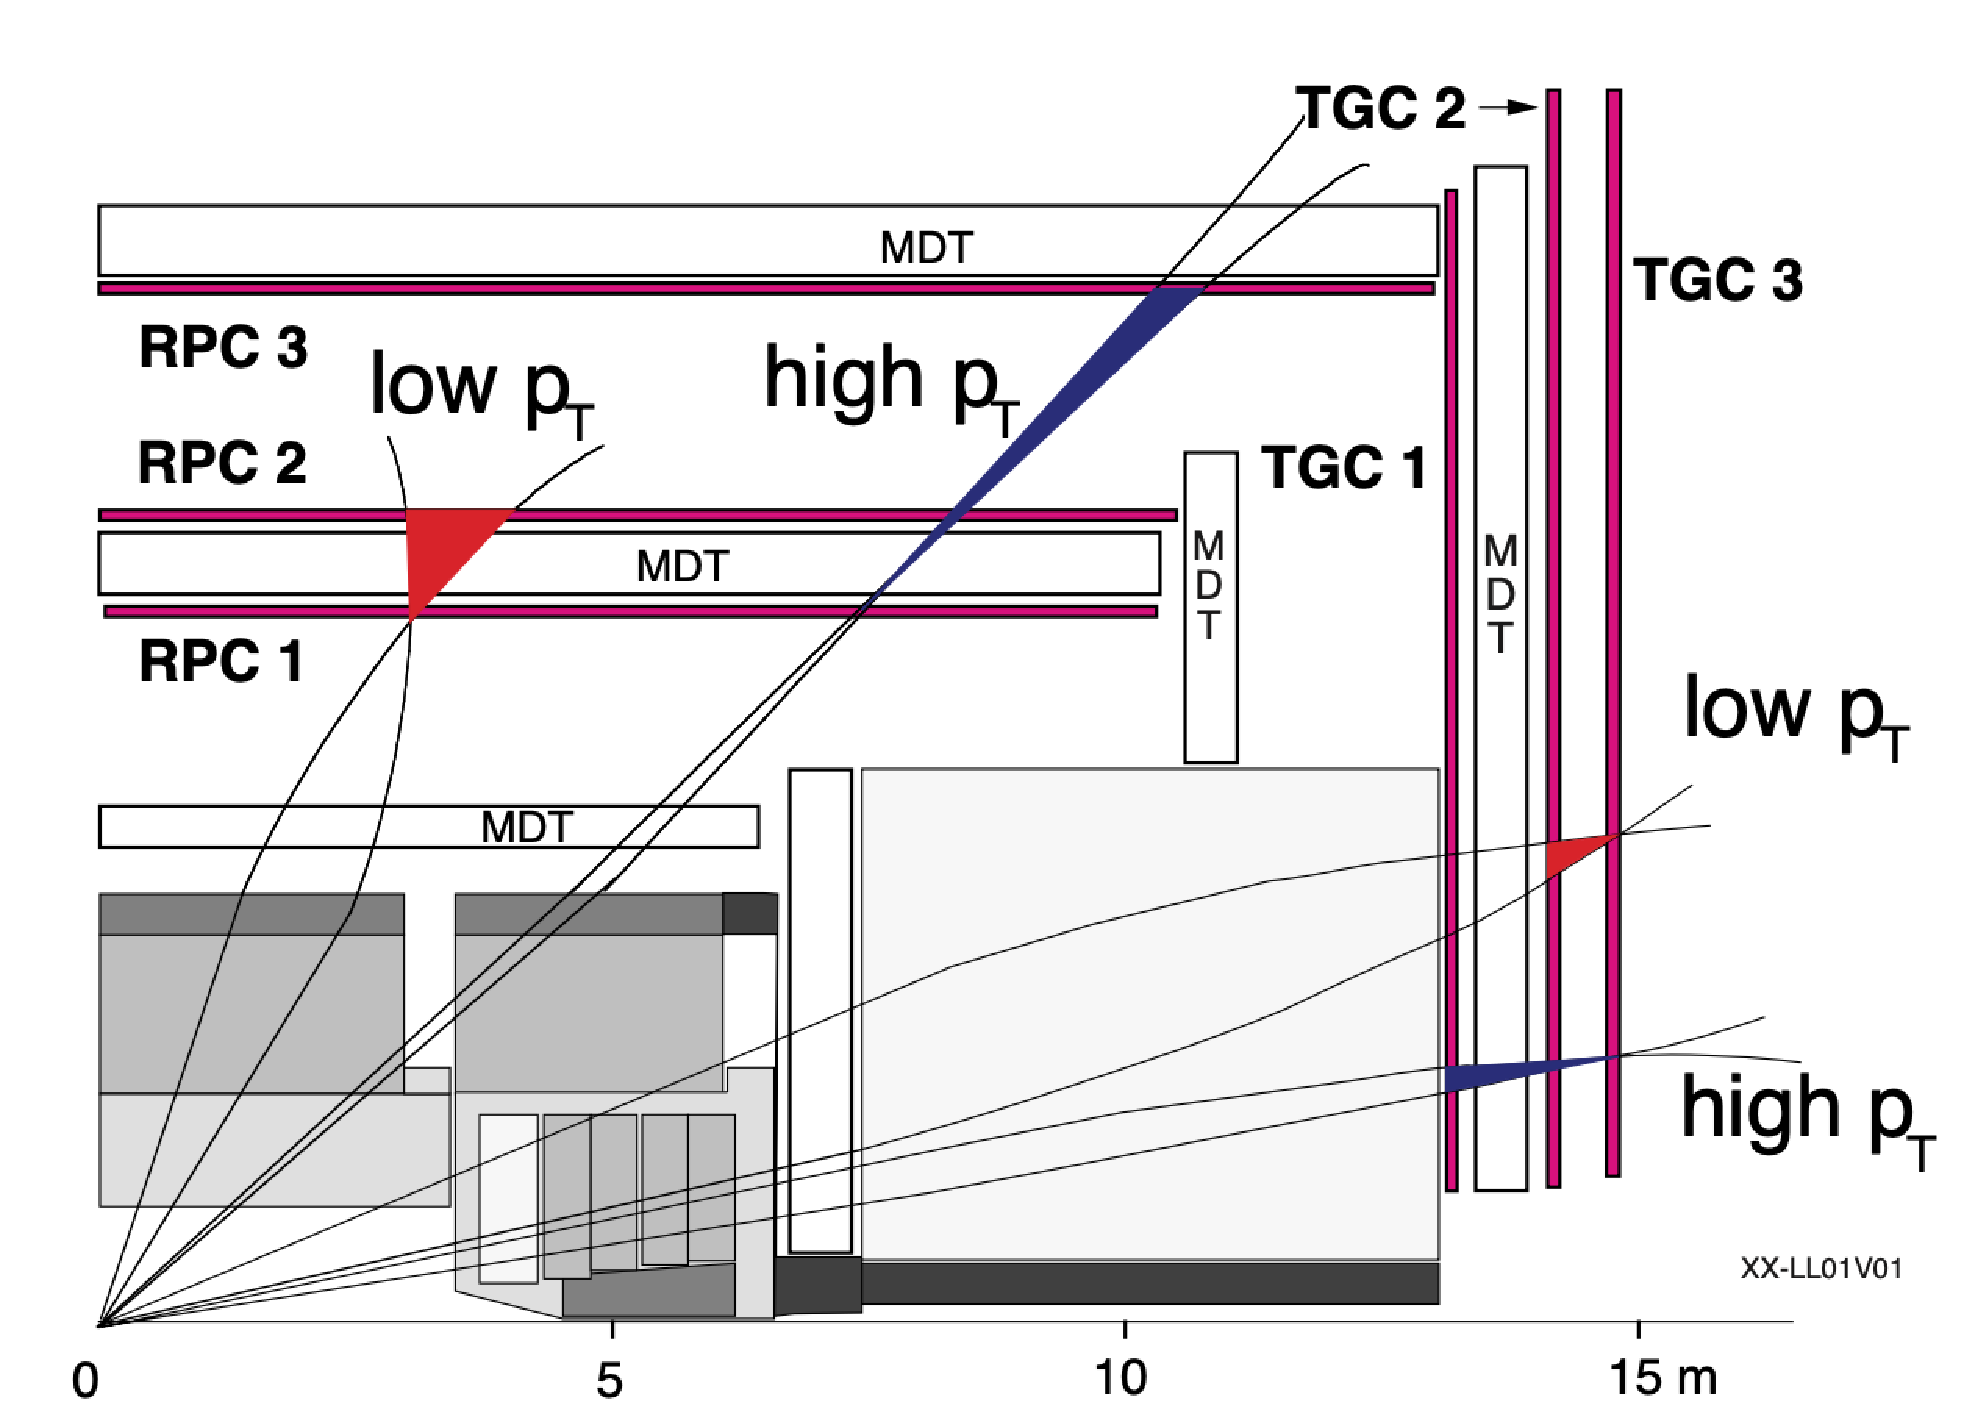
\includegraphics[width=0.95\textwidth]{figures/muontrigger/L1MuonTrigger.pdf}
	\caption{Longitudinal view of the barrel and end-cap muon trigger system. Representative tracks of muon trigger candidates for the low-\pt and high-\pt triggers illustrate the coincidence logic of trigger stations used for the trigger decision. Adapted from Ref.~\cite{CERN-LHCC-98-014}}.
	\label{fig:trigger:l1mu4:illustration}
\end{figure}

The barrel region is instrumented with three stations of Resistive Plate Chamber (RPC) detectors. RPCs are wireless strip detectors, consisting of two gas gaps designed for operation in saturated avalanche mode with planes of read-out strips in the transverse and longitudinal direction. They have an excellent timing \(\times\) position-resolution of \(\SI{1}{\nano\second} \times \SI{1}{\centi\meter}\) and a rate capability of \SI{10}{\kilo\hertz\per\square\centi\meter}. Two stations are located above (RPC2) and below (RPC1) the middle MDT layer. Coincidences between hits in the two layers define the muon track candidates. While the low-\pt trigger thresholds are based on the track candidates defined by the two innermost RPC layers, the high-\pt thresholds require additional coincidence with a third (RPC3) station, which is located below the outermost layer of MDT chambers. The RPC chambers provide information for the \(\eta\) and \(\phi\) coordinates of a muon track candidate.

The end-cap region is instrumented with Thin Gap Chamber (TGC) detectors. TGCs are multi-wire detectors consisting of a plane of closely spaced wires maintained at a positive high voltage enclosed by two resistive grounded cathode strip planes. The TGC chambers have excellent rate capability of more than \SI{30}{\kilo\hertz\per\square\centi\meter} and a better granularity than the RPC chambers, making them capable of operation in the end-cap region.
The TGCs are arranged in three planes in each end-cap at \(\abs{z} = \SI{14}{\meter}\). The innermost plane consists of three layers of TGCs (triplet unit), while the two outer planes consist of two layers of TGCs (doublet unit). The outermost plane is designed without gaps in acceptance or overlaps and constitutes the so-called pivot plane. Coincidences between hits in the pivot plane and the adjacent doublet plane, which is located in \SI{0.5}{\meter} distance, define the low-\pt trigger candidates. The trigger decision can be sharpened by requiring an additional coincidence with the triplet plane, which is located in \SI{1.6}{\meter} distance from the pivot plane. In particular, the high-\pt triggers make use of this requirement. The TGC wire channels provide information for the \(r\)-coordinate, while the TGC strip channels provide information for the \(\phi\)-coordinate of a muon track candidate.

A positive trigger decision associated with a certain \pt threshold requires the spatial coincidence to be consistent with the associated deviation from an infinite momentum track, thereby defining coincidence windows for the individual \pt thresholds. The coincidence windows are defined for the two projections in \(\eta\) and \(\phi\) (barrel) or \(r\) and \(\phi\) (end-cap), respectively.


\subsection{The L1MU4 coincidence logic tuning}
The L1MU4 muon trigger is designed to select muon candidates with \(\pt > \SI{4}{\giga\electronvolt}\).
The decision whether the \pt of the track is above the desired momentum threshold or not is based on coincidence windows, which are implemented as look-up-tables (LUTs).
The amount of deviation of the muon track candidate from an infinite momentum track in \(r\) and \(\phi\) is referred to as \(\Delta r\) and \(\Delta \phi\), respectively, and is used as input for the LUTs. For a given input of \(\Delta r\) and \(\Delta \phi\) the LUT determines a positive (pass) or negative (fail) trigger decision. A custom set of LUTs is defined for each region-of-interest (ROI) in each module of trigger chambers.

In Run-1, the L1MU4 employed a two-station full-open coincidence. In Run-2, a more sophisticated implementation is used, which uses requires three-station coincidence for the strip (\(\phi\)) coordinate and either two-station or three-station coincidence for the wire (\(r\)) coordinate. The LUT for the three-station wire (\(r\)) / three-station strip (\(\phi\)) coincidence is referred to as \textsc{HH CW}, whereas the two-station wire (\(r\)) / three-station strip (\(\phi\)) coincidence is referred to as \textsc{LH CW}.

The L1MU4 trigger rate can be reduced by tuning the LUTs, resulting in tighter coincidence windows for hits in the trigger chambers. This study investigates modifications affecting the forward trigger chambers, covering the pseudorapidity range \(2 < \abs{\eta} < 2.4\), by tuning the LH CW LUTs. A uniform modification of all LUTs corresponding to the 64 ROIs for the forward TGC modules 2a/b, 5a/b, and 8a/b is applied.
\Cref{fig:trigger:l1mu4:cw} shows the LUT implementation of the coincidence windows for a representative module of the detector end-cap before and after its optimisation.
Prior to the optimisation, all hits within two-station coincidence window of \(-15 \leq \Delta r \leq 15\) and the three-station coincidence window of \(-7 \leq \Delta \phi \leq 7\) resulted in a positive trigger decision.
After the optimisation, only hits within coincidence window of \(-7 \leq \Delta r \leq 7\) and \(-5 \leq \Delta \phi \leq 5\) resulted in a positive trigger decision.

\begin{figure}[htbp]
	\centering
	\begin{subfigure}[b]{0.45\textwidth}
		\centering
		\includegraphics[width=0.95\textwidth]{figures/muontrigger/l1mu4/cw_0025/cwplot_module2_roi0_pt1_cwHH.pdf}
		\caption{HH CW before optimisation}
	\end{subfigure}
	\begin{subfigure}[b]{0.45\textwidth}
		\centering
		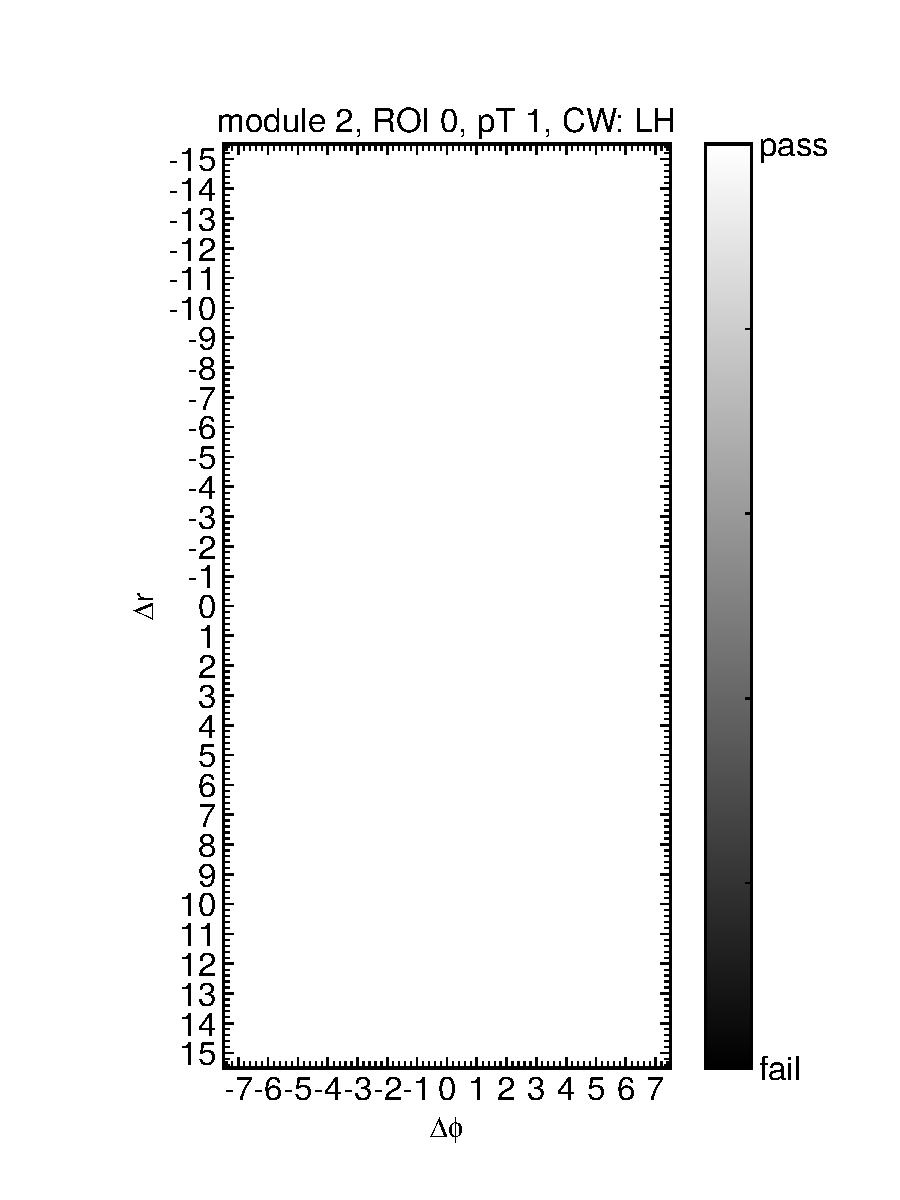
\includegraphics[width=0.95\textwidth]{figures/muontrigger/l1mu4/cw_0025/cwplot_module2_roi0_pt1_cwLH.pdf}
		\caption{LH CW before optimisation}
	\end{subfigure}
	\\
	\begin{subfigure}[b]{0.45\textwidth}
		\centering
		\includegraphics[width=0.95\textwidth]{figures/muontrigger/l1mu4/cw_0028/cwplot_module2_roi0_pt1_cwHH.pdf}
		\caption{HH CW after optimisation}
	\end{subfigure}
	\begin{subfigure}[b]{0.45\textwidth}
		\centering
		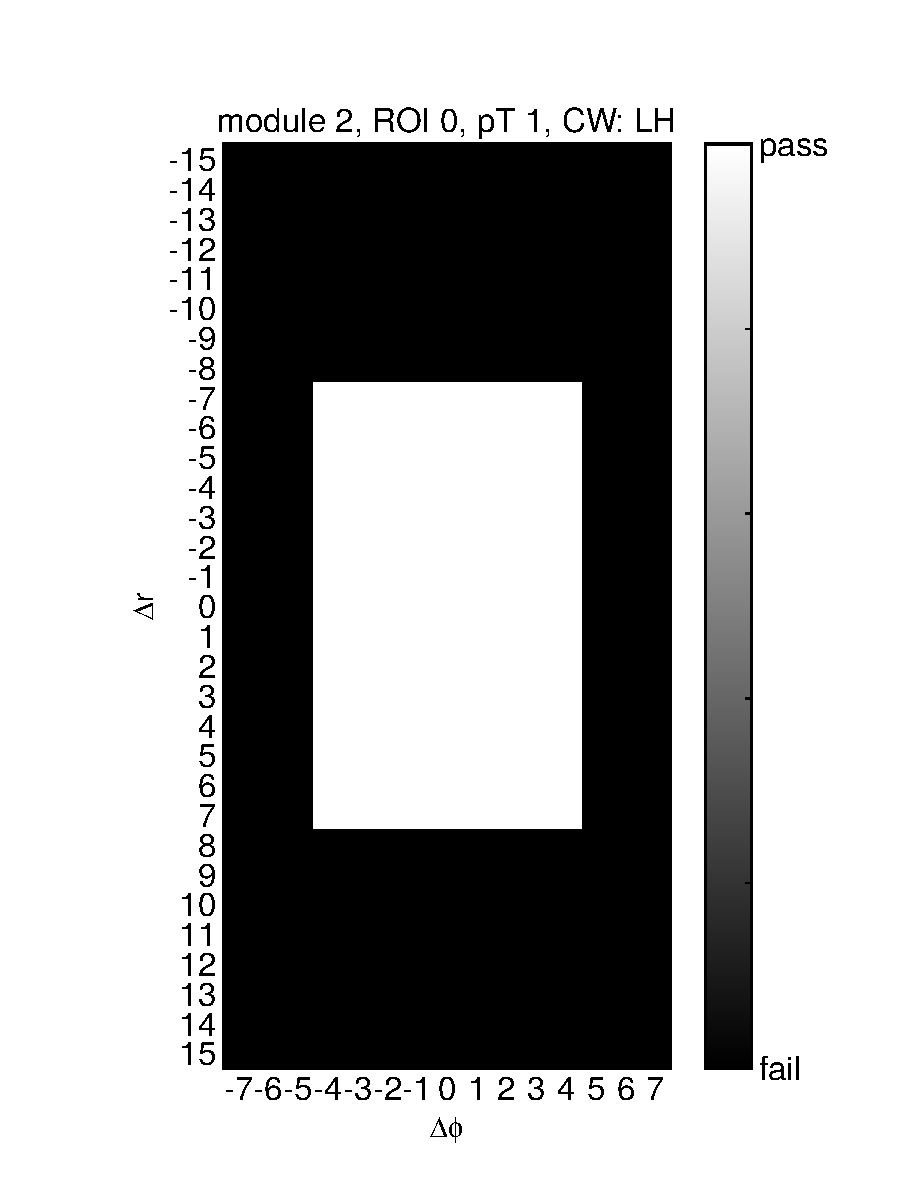
\includegraphics[width=0.95\textwidth]{figures/muontrigger/l1mu4/cw_0028/cwplot_module2_roi0_pt1_cwLH.pdf}
		\caption{LH CW after optimisation}
	\end{subfigure}

	\caption{Modification of coincidence windows in the \(\Delta r\)--\(\Delta \eta\) plane. The 0-th region-of-interest (ROI) LUTs for the HH CW and LH CW are shown for module 2a before (top row) and after (bottom row) the optimisation of the LH CW.}
	\label{fig:trigger:l1mu4:cw}
\end{figure}


\subsection{Data and method}
The effect of modifying the coincidence windows on the muon trigger efficiency is evaluated with a tag-and-probe method~\cite{Hensel2013,ATLAS-CONF-2012-099} based on the \PJpsi resonance into a pair of oppositely charged muons. The two muons are referred to as \emph{tag} and \emph{probe} muon. The \emph{tag} muon is the reconstructed muon, which fired the trigger for recording the event. The \emph{probe} muon is the other muon in the event. The \emph{probe} muons are used for an unbiased study whether a muon track candidate would fire the trigger for a given coincidence window definition. The muon trigger efficiency is estimated by

\begin{align}
    \varepsilon_{\mu-\text{trigger}} = \frac{N_{\text{match}}}{N_{\text{probe}}},
\end{align}

where \(N_{\text{match}}\) is the number of muon track candidates matched with a reconstructed muon within the \pt-dependent cone size of \(\Delta R\) in the \(\eta\)--\(\phi\) plane listed in \Cref{tab:trigger:l1mu4:dRmatching}, and \(N_{\text{probe}}\) is the total number of probe muons.

\begin{table}[!ht]
\caption{Cone size \(\Delta R\) used for matching the muon track candidate with a reconstructed muon in the \(\eta\)--\(\phi\), depending on the transverse momentum \pt and pseudorapidity \(\eta\) of the reconstructed muon.}
\label{tab:trigger:l1mu4:dRmatching}
\centering
\begin{tabular}{l l l}
\toprule
Minimum \pt of & \multirow{2}{*}{\(\Delta R\) (barrel)} & \multirow{2}{*}{\(\Delta R\) (end-cap)}\\
reconstructed muon & & \\
\midrule
 \SI{4}{\giga\electronvolt} & 0.3 & 0.3 \\
 \SI{6}{\giga\electronvolt} & 0.2 & 0.2 \\
\SI{10}{\giga\electronvolt} & 0.14 & 0.14 \\
\SI{15}{\giga\electronvolt} & 0.11 & 0.09 \\
\SI{20}{\giga\electronvolt} & 0.10 & 0.07 \\
\bottomrule
\end{tabular}
\end{table}

The tag-and-probe muon pairs are selected in data by the requirements listed in \Cref{tab:trigger:l1mu4:eventselection}. The muons are required to have opposite charge, and their invariant mass has to be consistent with the \PJpsi resonance.

\begin{table}[!ht]
\caption{Event selection requirements}
\label{tab:trigger:l1mu4:eventselection}
\centering
\begin{tabular}{ll}
\toprule
Event selection & Requirement \\
\midrule
Trigger & pass \textsc{HLT\_noalg\_L1MU4} \\
Muon multiplicity & \(N_{\mu} \geq 2 \) \\
Muon pair invariant mass & \(\SI{2.7}{\giga\electronvolt} < m_{\mu\mu} < \SI{3.5}{\giga\electronvolt}\) \\
Muon pair opposite charge & \(q_{\text{tag}} \times q_{\text{probe}} < 0\) \\
\bottomrule
\end{tabular}
\end{table}

The reconstructed muons are subject to quality requirements listed in \Cref{tab:trigger:l1mu4:objectselection}.
Their pseudorapidity \(\eta\) is required to be within the trigger chamber acceptance of \(\abs{\eta} < 2.4 \). Muons are required to be reconstructed with either \emph{Medium} or \emph{High-\pt} working point, as defined in Ref.~\cite{PERF-2015-10}. Specific requirements on the number of hits in the inner detector of the reconstructed ensure a robust momentum measurement.
Additional requirements are placed on the \emph{tag} muon, which has to satisfy \(\pt > \SI{4}{\giga\electronvolt}\) and has to be matched with the muon track candidate of a single muon trigger within \(\Delta R < 0.05\) in the \(\eta\)--\(\phi\) plane.

\begin{table}[!ht]
\caption{Selection requirements on tag and probe muons}
\label{tab:trigger:l1mu4:objectselection}
\centering
\begin{tabular}{ll}
\toprule
Reconstructed muons       & Quality requirement \\
\midrule
                          & \(\abs{\eta} < 2.4\) \\
						  & Medium or High-\pt working point \\
        				  & 1 or more hits in PXD detector \\
        				  & 4 or more hits in SCT detector \\
        				  & 1 or more hits in Pixel detector \\
        				  & 2 or less holes in PXD + SCT detectors \\
\midrule
Tag muon       & Additional quality requirement \\
\midrule
               & \(\pt > \SI{4}{\giga\electronvolt}\) \\
               & matched with single-lepton trigger by requiring \\
               & \(\Delta R(\mu, \text{muon trigger track candidate}) < 0.05\) \\
\bottomrule
\end{tabular}
\end{table}

The data for the efficiency study was taken in 2016 and amounts to over \num{159264525} recorded collision events.
The kinematic distributions of the selected \emph{tag} and \emph{probe} muon pairs and their invariant mass is shown in \Cref{fig:trigger:l1mu4:kinematics}. The threshold structure in the muon \pt distribution is due to limited bandwidth of the low-\pt muon triggers. The structure of the \(\eta\) distribution is due to gaps in the detector acceptance at the central maintenance shaft and the transition region between barrel and end-cap.
The reduced acceptance for \(\phi = -1.1\) and \(\phi = -2.0\) originates from the inferior instrumentation in the feet region of the ATLAS detector.

\begin{figure}[htbp]
	\centering
	\begin{subfigure}[b]{0.45\textwidth}
		\centering
		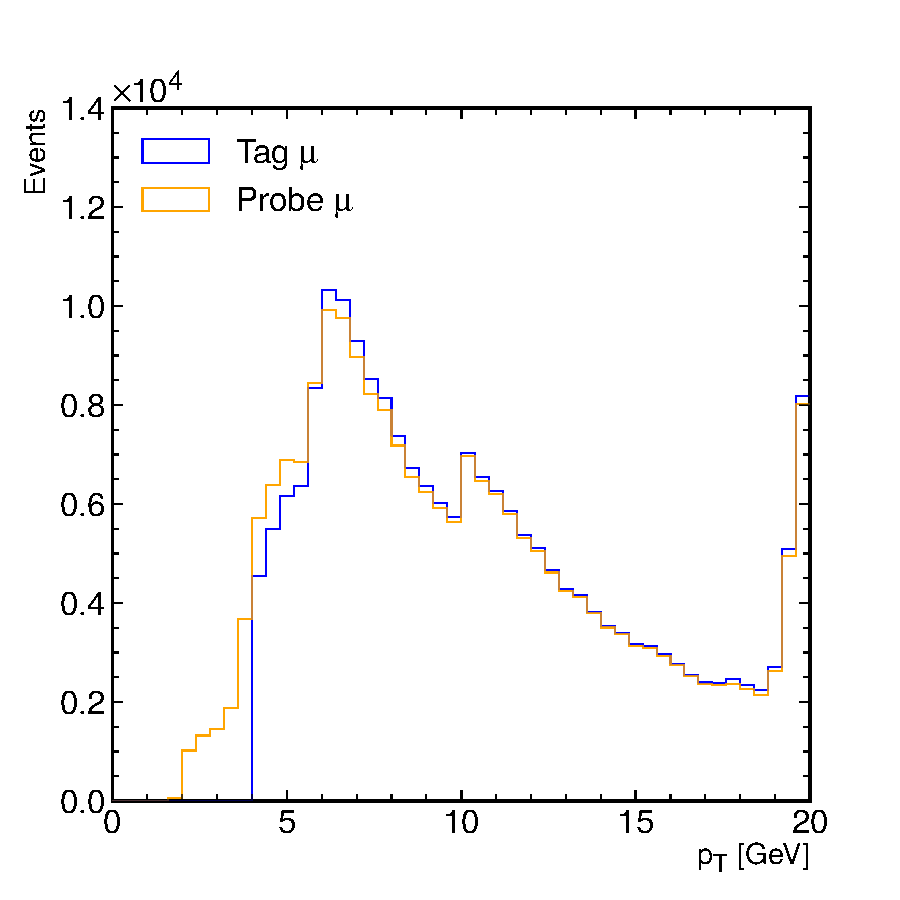
\includegraphics[width=0.95\textwidth]{figures/muontrigger/l1mu4/l1mu4_muon_pt.pdf}
		\caption{Muon transverse momentum \pt}
	\end{subfigure}
	\begin{subfigure}[b]{0.45\textwidth}
		\centering
		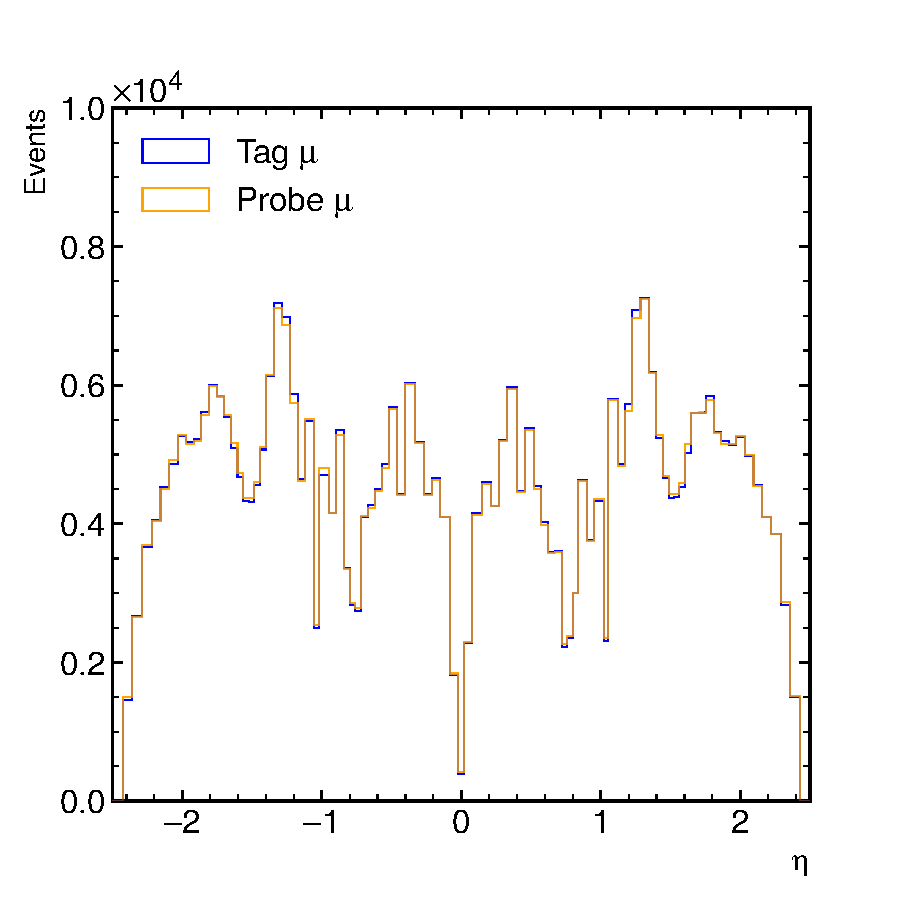
\includegraphics[width=0.95\textwidth]{figures/muontrigger/l1mu4/l1mu4_muon_eta.pdf}
		\caption{Muon pseudorapidity \(\eta\)}
	\end{subfigure} \\

	\begin{subfigure}[b]{0.45\textwidth}
		\centering
		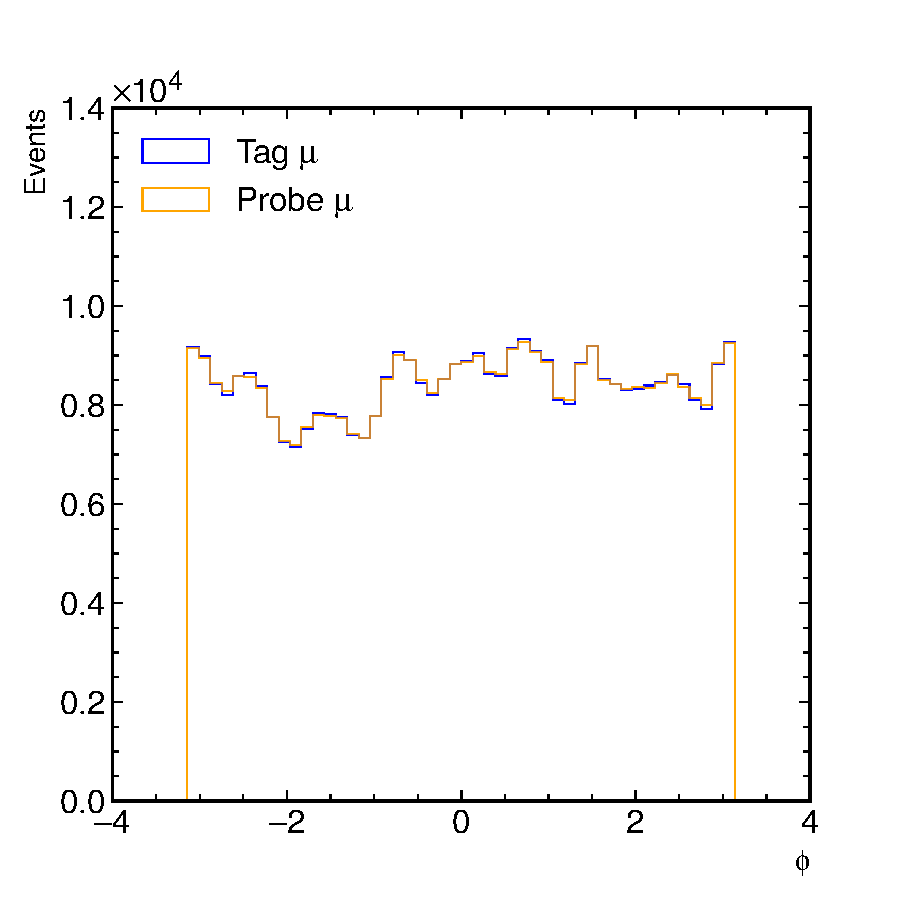
\includegraphics[width=0.95\textwidth]{figures/muontrigger/l1mu4/l1mu4_muon_phi.pdf}
		\caption{Muon azimuthal coordinate \(\phi\)}
	\end{subfigure}
	\begin{subfigure}[b]{0.45\textwidth}
		\centering
		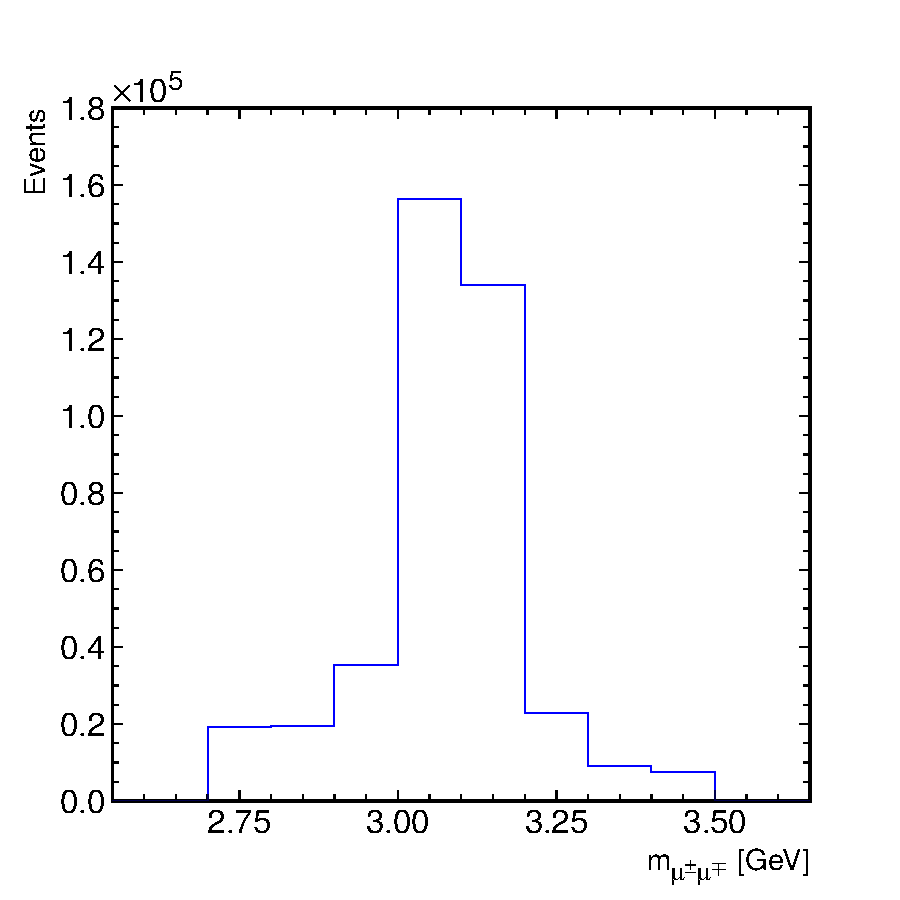
\includegraphics[width=0.95\textwidth]{figures/muontrigger/l1mu4/l1mu4_dimuon_mass.pdf}
		\caption{Invariant mass of muon pair}
	\end{subfigure}

	\caption{Kinematic distributions of \emph{tag} and \emph{probe} muons and invariant mass of the di-muon system after the full event selection.}
	\label{fig:trigger:l1mu4:kinematics}
\end{figure}



\subsection{Results}
Modifications to the coincidence windows of the end-cap trigger stations result in a \SI{4.5}{\percent} reduction of the trigger rate while maintaining a muon efficiency of \SI{99.8}{\percent}.

\Cref{fig:trigger:l1mu4:efficiency} shows the L1MU4 trigger efficiency before and after the optimisation of the forward module coincidence windows. The coincidence window optimisation has an almost negligible effect on the L1MU4 trigger efficiency. Only for the muons in the forward region \(2.0 < \abs{\eta} < 2.4\) with \(\pt < \SI{5}{\giga\electronvolt}\), a drop in trigger efficiency in the sub-percent-range is observed. The overall impact of the modification on the L1MU4 trigger efficiency is sufficiently small not to impact the performance of the L1MU4 trigger.

\begin{figure}[htbp]
	\centering
	\begin{subfigure}[b]{0.45\textwidth}
		\centering
		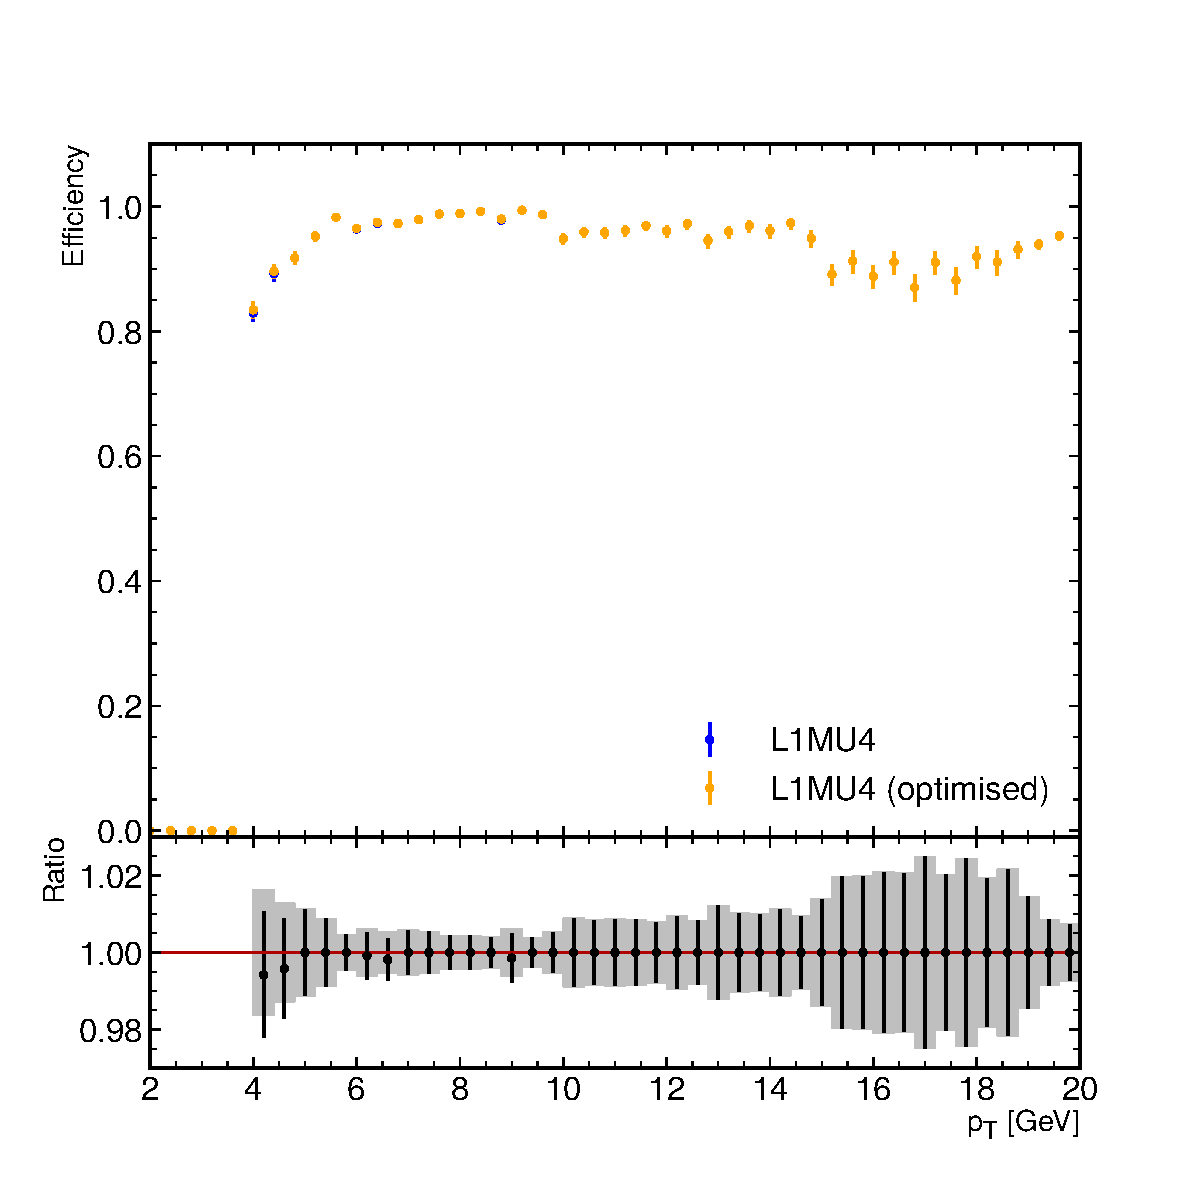
\includegraphics[width=0.95\textwidth]{figures/muontrigger/l1mu4/l1mu4_eff_pt_forward.pdf}
		\caption{Trigger efficiency vs. muon track candidate \pt for \(2.0 < \abs{\eta} < 2.4\)}
	\end{subfigure}
	\begin{subfigure}[b]{0.45\textwidth}
		\centering
		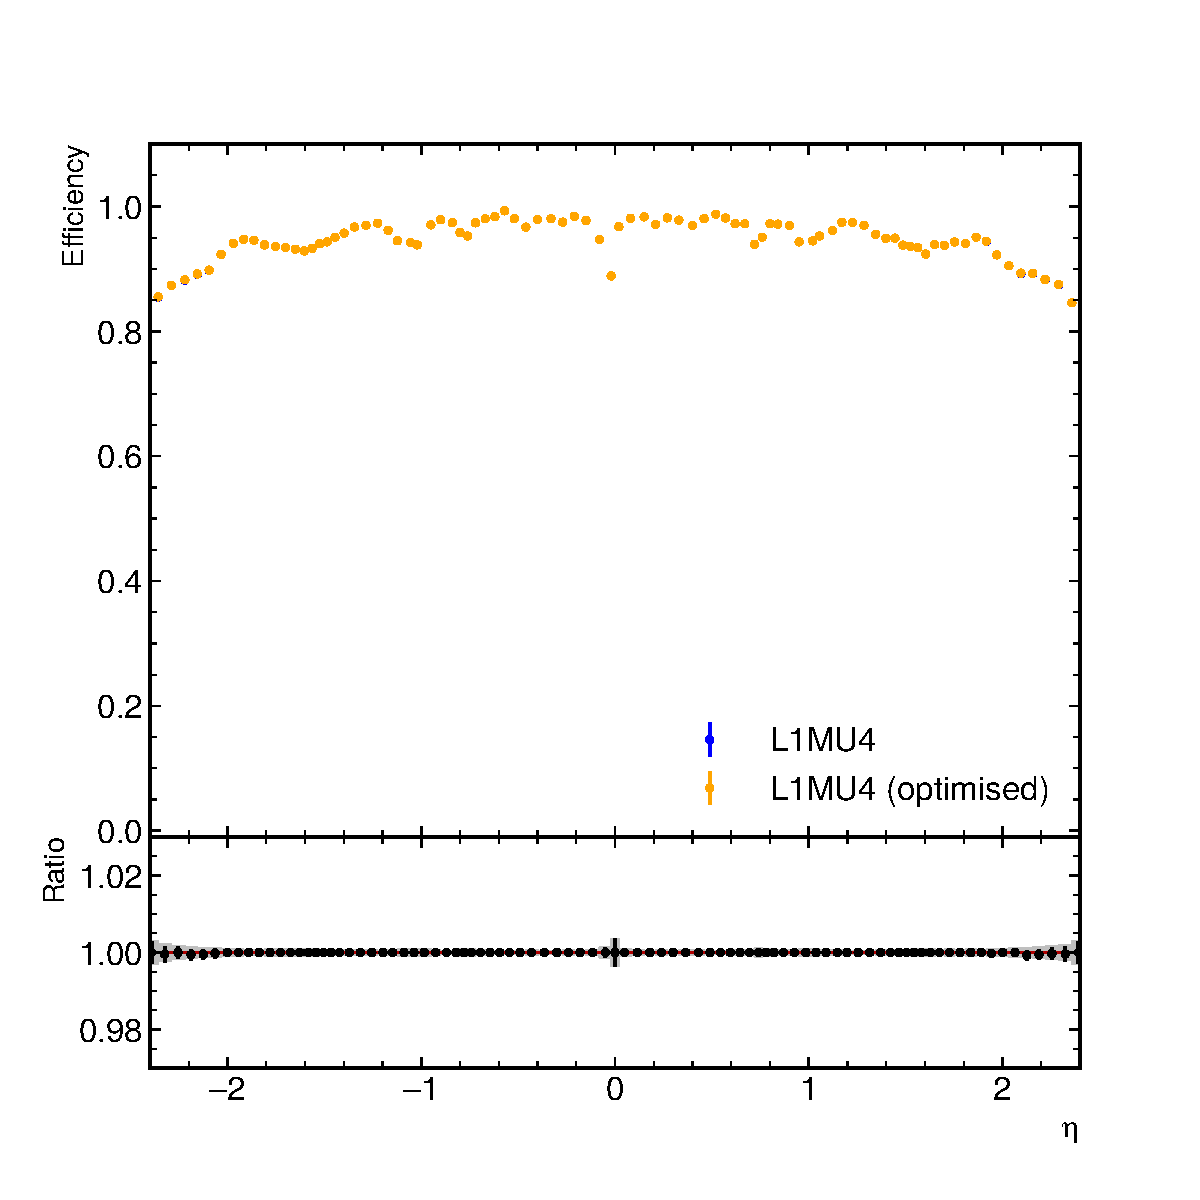
\includegraphics[width=0.95\textwidth]{figures/muontrigger/l1mu4/l1mu4_eff_eta.pdf}
		\caption{Trigger efficiency vs. muon track candidate \(\eta\)}
	\end{subfigure}

	% removed due to space constraints
	% \begin{subfigure}[b]{0.45\textwidth}
	% 	\centering
	% 	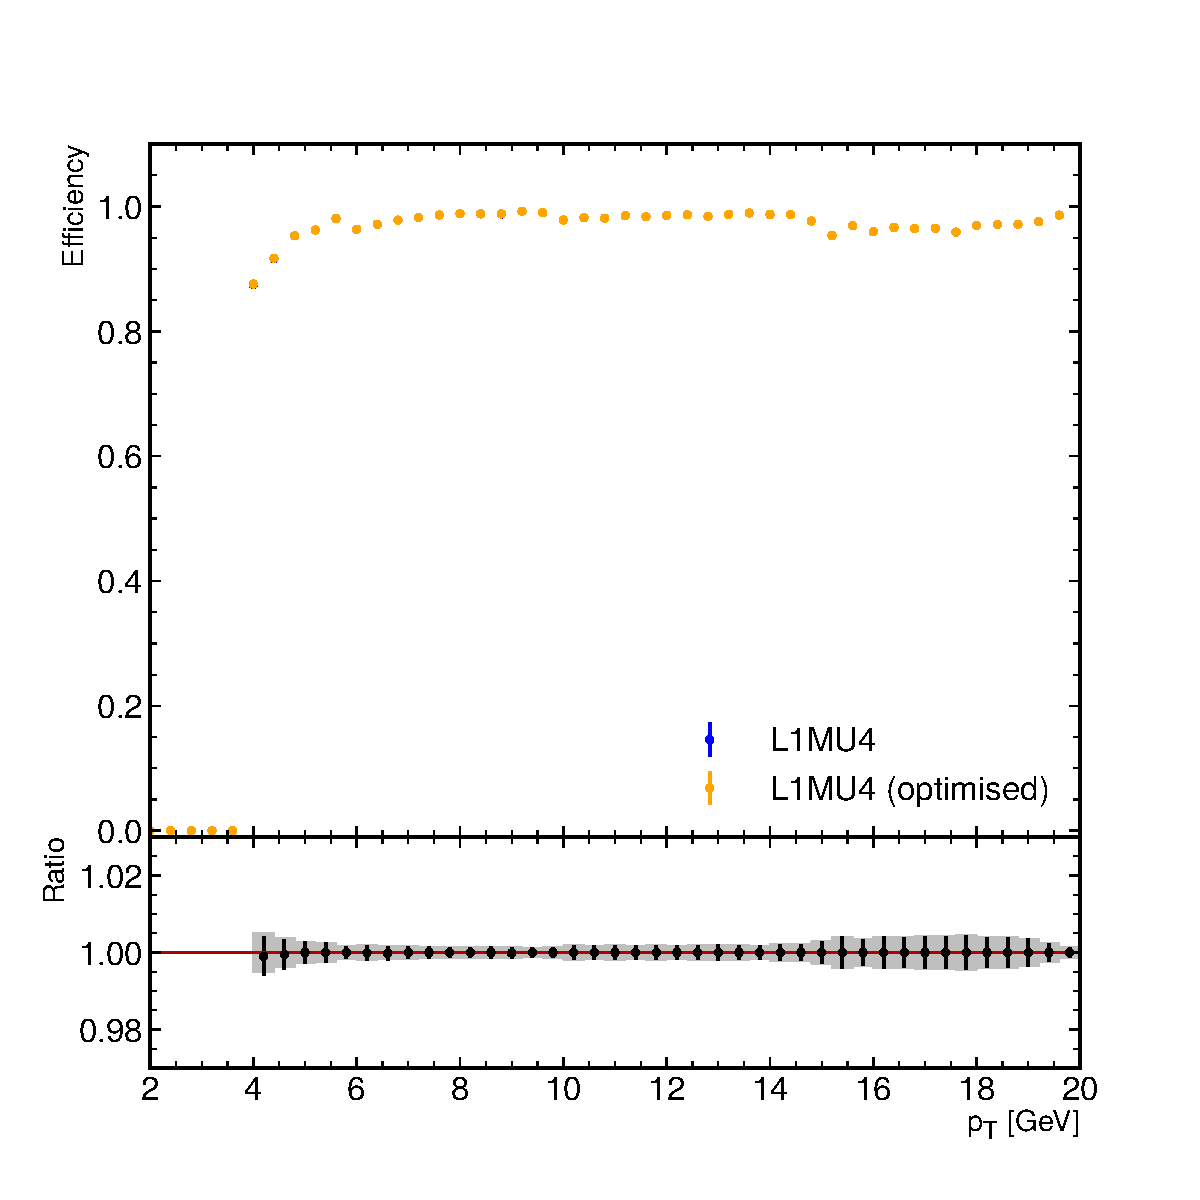
\includegraphics[width=0.95\textwidth]{figures/muontrigger/l1mu4/l1mu4_eff_pt_all.pdf}
	% 	\caption{Trigger efficiency vs. muon track candidate \pt for full \(\eta\) range}
	% \end{subfigure}
	% \begin{subfigure}[b]{0.45\textwidth}
	% 	\centering
	% 	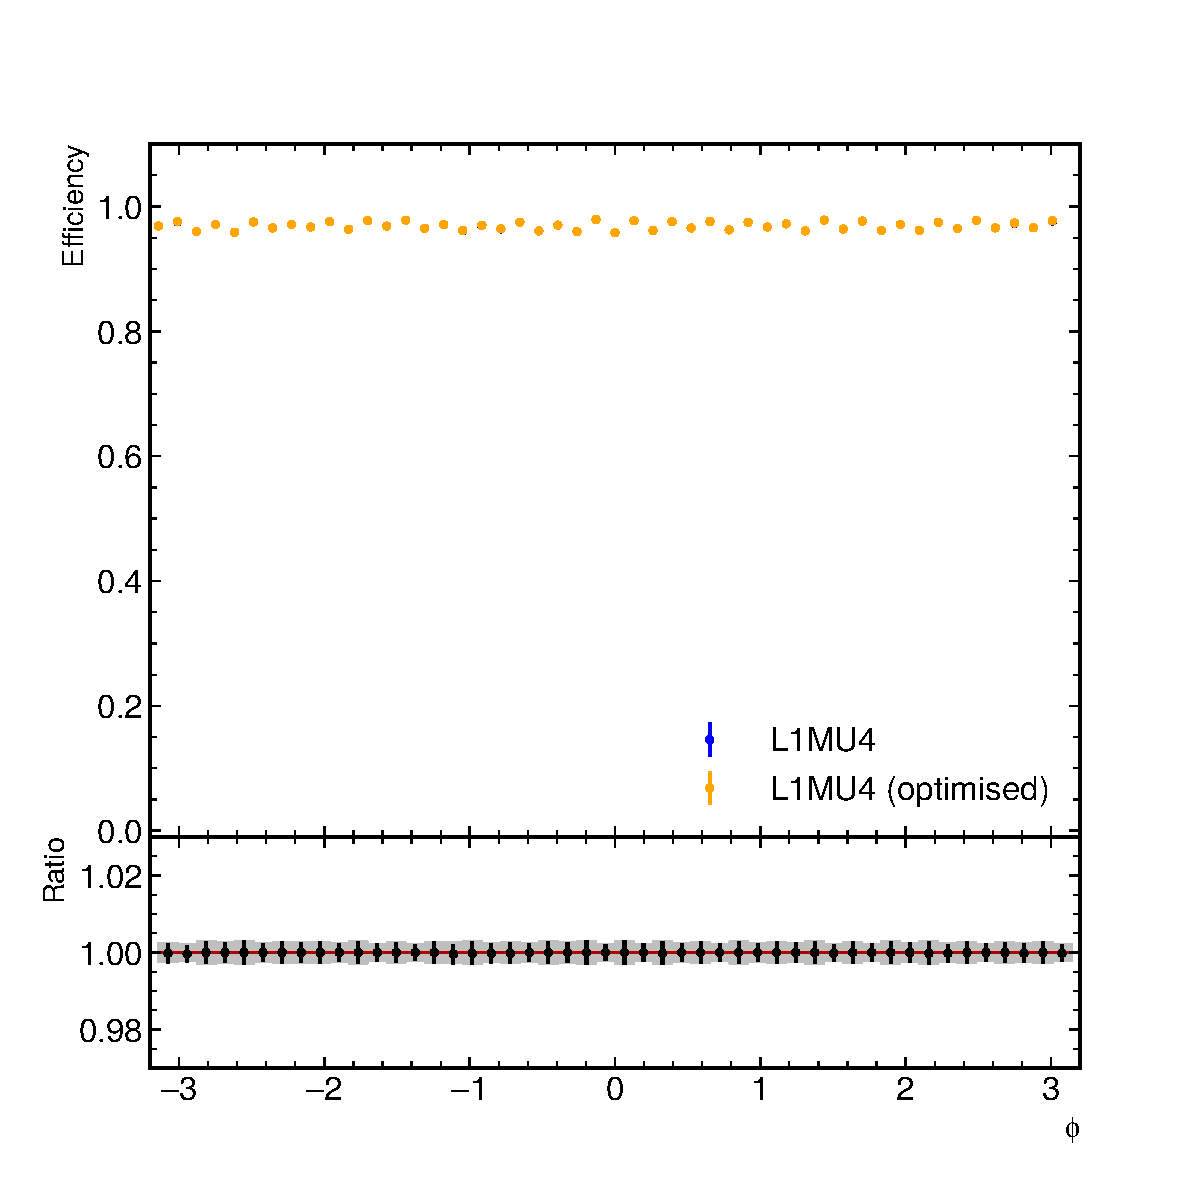
\includegraphics[width=0.95\textwidth]{figures/muontrigger/l1mu4/l1mu4_eff_phi.pdf}
	% 	\caption{Trigger efficiency vs. muon track candidate \(\phi\)}
	% \end{subfigure}

	\caption{L1MU4 trigger efficiency before and after the optimisation of the forward module coincidence windows estimated with the tag-and-probe method based on the \PJpsi resonance.}
	\label{fig:trigger:l1mu4:efficiency}
\end{figure}


The reduction in the muon trigger rate is shown in \Cref{fig:trigger:l1mu4:rate} in dependency of the pseudorapidity \(\eta\) of the muon track candidate. The modification of the LUTs for the forward modules (\(2.0 < \abs{\eta} < 2.4\)) resulted in a decrease of the trigger rate without affecting the rate of triggers matched to reconstructed muons. In the forward region \(2.0 < \abs{\eta} < 2.4\), the L1MU4 trigger rate is reduced by \SI{20}{\percent} while maintaining a muon efficiency of \SI{99.0}{\percent}.

\begin{figure}[htbp]
	\centering
	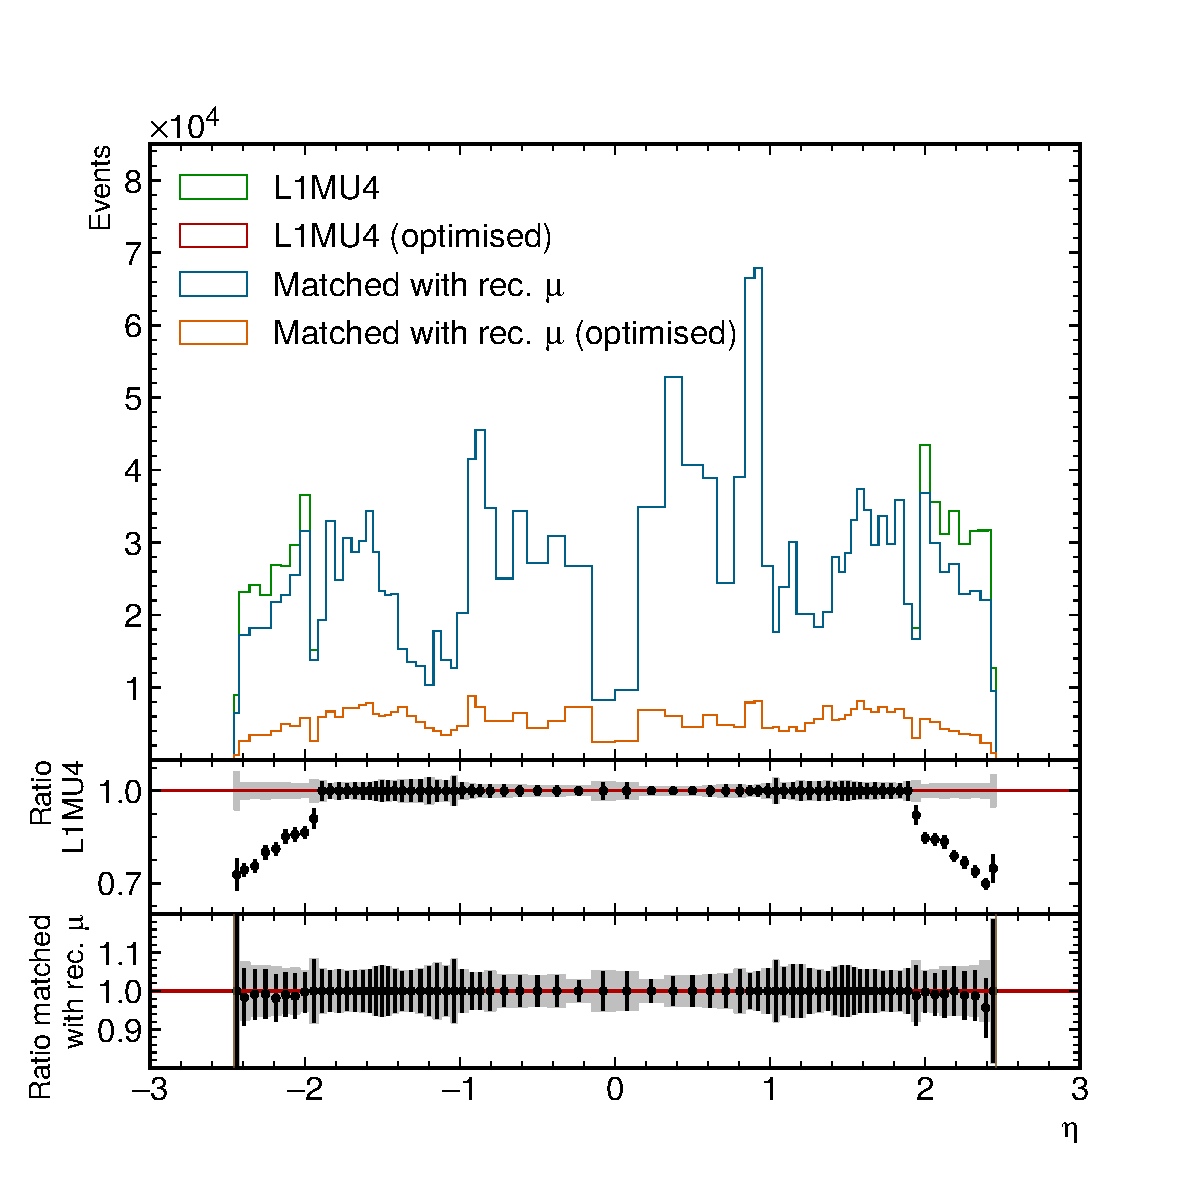
\includegraphics[width=0.95\textwidth]{figures/muontrigger/l1mu4/l1mu4_rate_eta.pdf}
	\caption{L1MU4 trigger rate in dependency of the muon track candidate pseudorapidity \(\eta\) before and after the optimisation of the coincidence windows of the forward TGC modules. In addition, the rate of positive trigger decisions which could be matched with a reconstructed muon satisfying \(\pt > \SI{4}{\giga\electronvolt}\) is shown before and after the coincidence window modification. The two insets show the ratio of the L1MU4 trigger rate after and before the coincidence window modification and the ratio of positive trigger decisions matched with reconstructed muons after and before the coincidence window modification, respectively.}
	\label{fig:trigger:l1mu4:rate}
\end{figure}

The reduction of the trigger rate and the effect on the trigger efficiency for triggers with multiple muons is shown in \Cref{tab:trigger:l1mu4:results}. For events with two (three) or more muon track candidates leading to a positive trigger decision, the optimised coincidence windows result in a reduction of the L1MU4 trigger rate by \SI{6}{\percent} (\SI{9}{\percent}), while keeping \SI{99.2}{\percent} (\SI{100}{\percent}) of the muon trigger efficiency.

\begin{table}[!ht]
\caption{Effect of the coincidence window optimisation in the forward TGC modules on the L1MU4 trigger rate and trigger efficiency \(\varepsilon\) for muon triggers with different muon multiplicities.}
\label{tab:trigger:l1mu4:results}
\centering
\begin{tabular}{l rr }
\toprule
                          & L1MU4 rate reduction & \(\varepsilon_{\text{L1MU4, mod.}} / \varepsilon_{\text{L1MU4}}\)\\
\midrule
1 or more muon track candidate & \SI{5}{\percent} & \SI{99.8}{\percent} \\
2 or more muon track candidates & \SI{6}{\percent} & \SI{99.2}{\percent} \\
3 or more muon track candidates & \SI{9}{\percent} & \SI{100}{\percent} \\
\bottomrule
\end{tabular}
\end{table}
